\chapter{Widgets}

Everything in Flutter is a Widget. This incorporates UI components, like ListView,
TextBox, and Image, just as different parts of the system, including format, activity, motion
acknowledgment, and subjects, to give some examples.\\
Widgets are fundamental for an application's view and interface. They should have a characteristic look and
feel paying little heed to screen size. They likewise should be quick, extensible, and adjustable. Flutter takes the
Everything is a Widget approach. It has a rich arrangement of Widgets and broad abilities for making
complex custom Widgets. In Flutter, Widgets aren't just utilized for views. They're additionally utilized for whole
screens and in any event, for the actual application.\\
As Flutter's documentation puts it, every Widget is an unchanging presentation of part of the
UI. Different structures separate perspectives, view regulators, designs, and different properties.
Flutter, then again, has a predictable, consistent, brought together item model: the Widget.
A Widget can characterize an underlying component (like a button or menu); a complex component (like a textual style
or on the other hand color scheme); a part of the format (like padding, etc.
Widgets structure a chain of command dependent on their piece. Every Widget settles within and acquires
properties from its parent. There's no different application object. All things considered, the root Widget serves this
job.\\
Flutter has a full arrangement of Widgets in Google's Material Design and in Apple's style with the
Cupertino pack. Widget delivering happens straightforwardly in the Skia engine without utilizing Original
Equipment Manufacturer Widgets. So we get a smoother UI experience contrasted and other cross
platform structures.\\
\\
Widgets in Flutter are divided into two sub categories:\\
1) StateLess Widgets\\
2) StateFul Widgets\\

\section{StateLess Widgets}

A stateless Widget is a Widget that portrays part of the UI by building a network 
of different Widgets that portray the UI all the more solidly. The building process proceeds
recursively until the description of the UI is completely concrete.\\
\begin{figure}[h]
  \begin{center}
  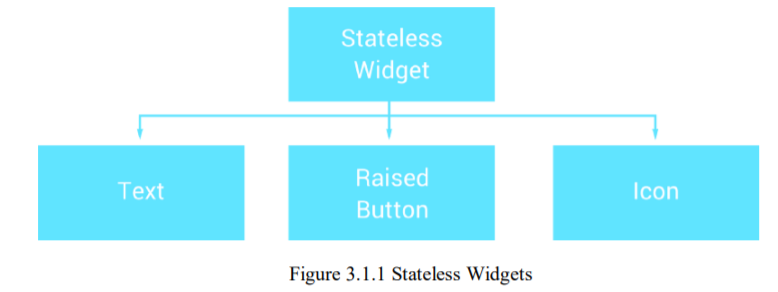
\includegraphics[height=55mm]{Images & Logos/CH_03_STATELESS.png}\\
  \end{center}
  \caption{Stateless Widget}
\end{figure}  

Stateless Widget are valuable when the piece of the UI you are portraying doesn't rely upon something besides the arrangement data in the actual article and the BuildContext in which the Widget is expanded. For compositions that can change dynamically, for example due to having an inside clock-driven state, or relying upon some system state, think about utilizing StatefulWidget.\\

\section{StateFul Widget}
A stateful widget is a widget that describes part of the user interface by building a constellation of other widgets that describe the user interface more concretely. The building process continues recursively until the description of the user interface is fully concrete (e.g., consists entirely of RenderObjectWidgets, which describe concrete RenderObjects).\\

\begin{figure}[h]
  \begin{center}
 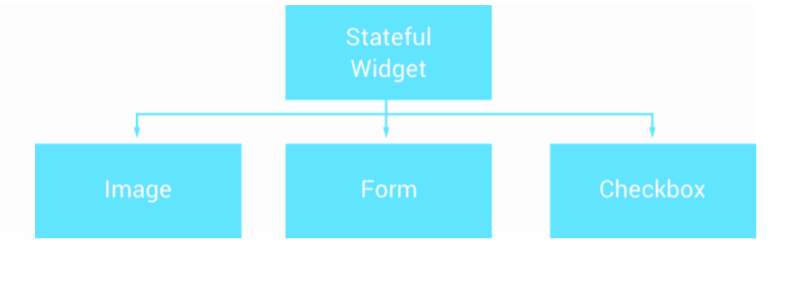
\includegraphics[height=55mm]{Images & Logos/CH_03_STATEFUL.png}
  \end{center}
  \caption{Stateful Widget}
\end{figure}  
Stateful widgets are useful when the part of the user interface you are describing can change dynamically, e.g. due to having an internal clock-driven state, or depending on some system state. For compositions that depend only on the configuration information in the object itself and the BuildContext in which the widget is inflated, consider using StatelessWidget.\\
